% vim:encoding=utf8 ft=tex sts=2 sw=2 et:

\documentclass{classrep}
\usepackage[utf8]{inputenc}
\usepackage{fixltx2e}
\usepackage{url}
\usepackage{graphicx}
\usepackage{siunitx}


\studycycle{Informatyka, studia niestacjonarne, inż I st.}
\coursesemester{VI}

%\coursename{hhhhhhhheoretyczna i stosowana}
\coursename{Inteligentna Analiza Danych}
\courseyear{2013/2014}

\courseteacher{mgr inż. Michał Pryczek}
\coursegroup{sobota, 11:15}

\author{
  \studentinfo{Łukasz Ochmański}{183566} \and
  \studentinfo{Przemysław Szwajkowski}{173524}
}

\title{Zadanie 3: Sieci samoorganizujące się działające na zasadzie współzawodnictwa}
\svnurl{http://iad-lukasz-ochmanski.googlecode.com/svn/trunk/03}

\begin{document}
\maketitle


\section{Cel}
Zadaniem zespołu laboratoryjnego jest przebadanie cech zadania grupowania danych. W tym celu zespół zobowiązany jest:
\begin{enumerate}
    \item Stworzyć implementację algorytmu k-średnich
		\item Stworzyć implementację neuronowej samoorganizującej się mapy w jednym z wariantów metody jej nauki.
\\
\\
Obowiązkowe warianty algorytmu uczenia sieci:
\begin{enumerate}
		\item Algorytm Kohonena
		\item Algorytm gazu neuronowego
		\\
\end{enumerate}
\end{enumerate}


\par
Sieć realizująca klasyczną samoorganizującą się mapę składa się ze zbioru neuronów, których układ może być rozpatrywany jako pojedyncza warstwa. Neurony rywalizują za sobą o prawo do reprezentowania wzorca wejściowego- w tym sensie ten który odpowie najsilniej jest ostatecznie przyjmowany jako reprezentant wzorca. Funkcja transmisji neuronów jest przeważnie (i takiej należy użyć rozwiązując niniejsze zadanie) funkcją odległości między wektorem wejściowym a wektorem wag- w tym układzie nie uwzględniamy również biasu, a dany neuron możemy zinterpretować jako punkt/wektor w przestrzeni wzorców wejściowych. Osobną kwestią jest znalezienie optymalnego rozkładu neuronów w przestrzeni. 

\section{Wstęp}
W badaniu uwzględniono trzy zbiory danych wygenerowane na stronie:
\\
http://hydra.ics.p.lodz.pl/data
\\
\begin{itemize}
\item
Zbiór nr 1: kolumny 0, 1
\item
Zbiór nr 2: kolumny 2, 3, 4
\item
Zbiór nr 3: kolumny 5, 6, 7
\\
\\
\end{itemize}

\par

\begin{figure}[h]
	\centering
		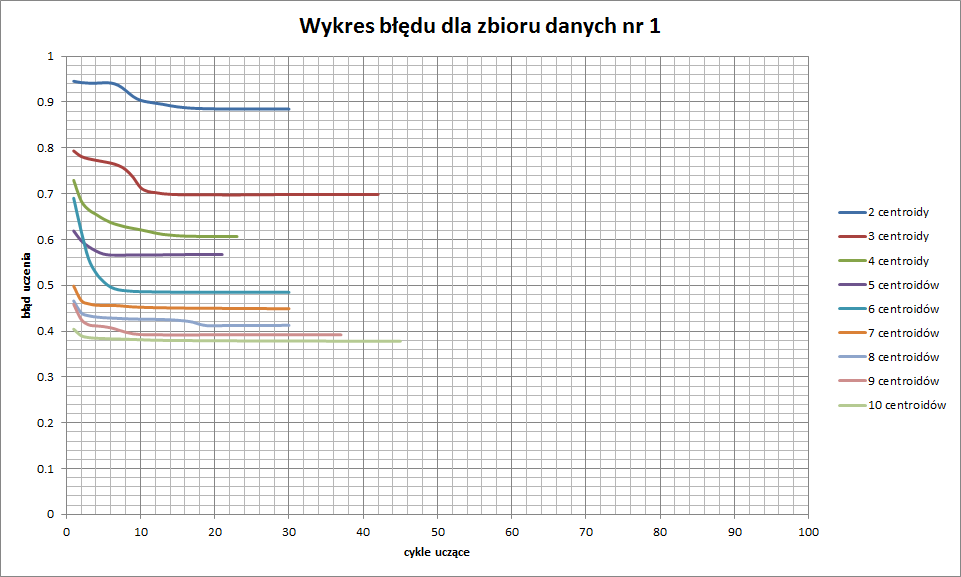
\includegraphics[scale=0.55]{pictures/183566_kmeans_1.png}
	\caption{Adaptacyjny dobór wartości k dla zbioru nr 1}
	\label{fig:183566_kmeans_1}
\end{figure}


\begin{figure}[h]
\centering
			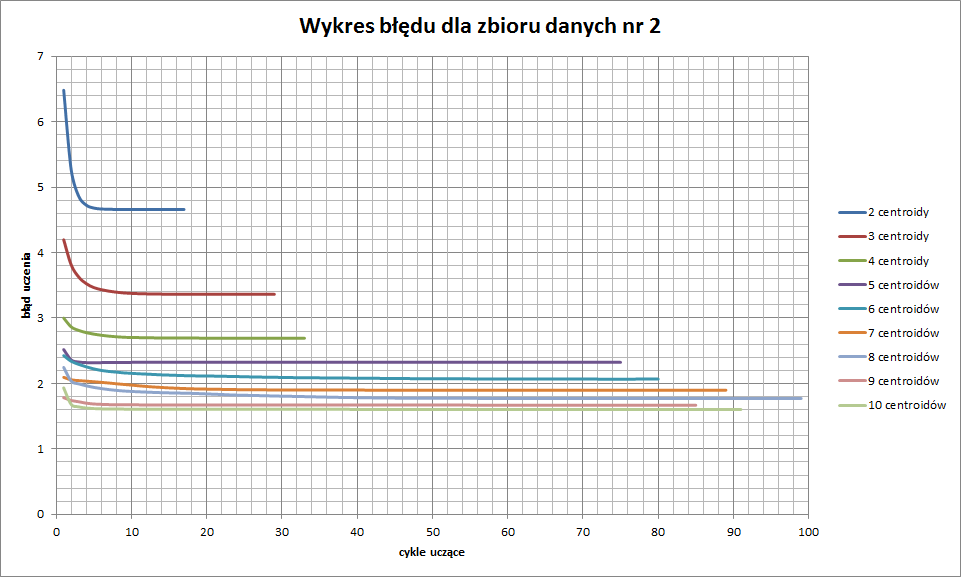
\includegraphics[scale=0.55]{pictures/183566_kmeans_2.png}
	\caption{Adaptacyjny dobór wartości k dla zbioru nr 2}
	\label{fig:183566_kmeans_2}
\end{figure}

\clearpage

\begin{figure}[h]
\centering
			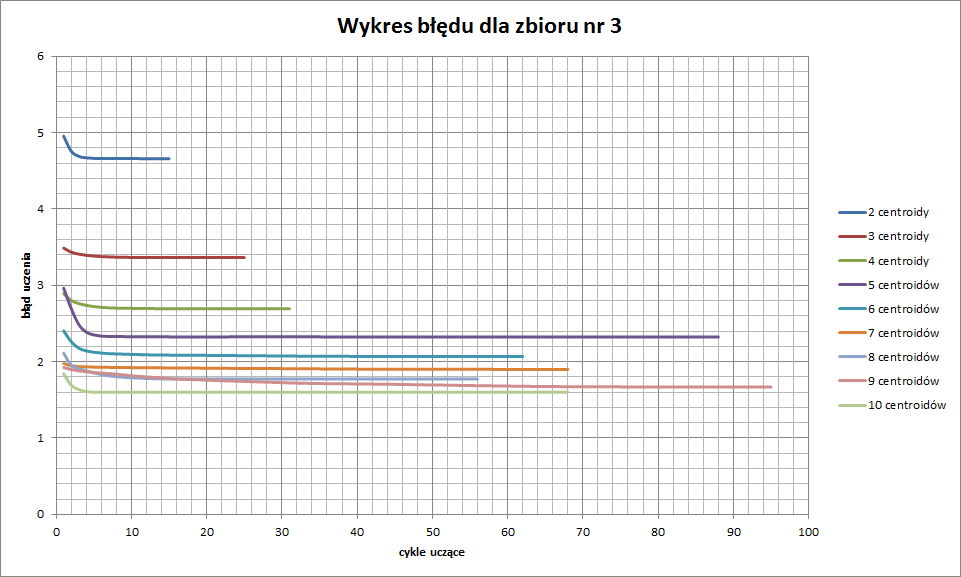
\includegraphics[scale=0.55]{pictures/183566_kmeans_3.png}
	\caption{Adaptacyjny dobór wartości k dla zbioru nr 3}
	\label{fig:183566_kmeans_3}
\end{figure}

Jak widać na wszystkich wykresach błąd uczenia sieci jest najmniejszy dla największej liczby centroidów.
\clearpage

\begin{figure}[h]
	\centering
		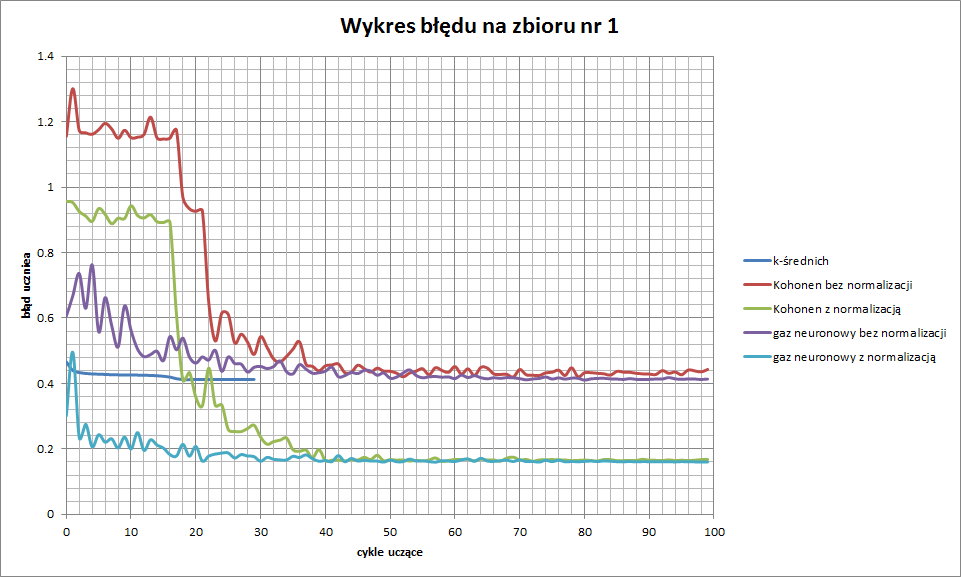
\includegraphics[scale=0.55]{pictures/183566_1.png}
	\label{fig:183566_1}
	\caption{Porównanie błędu uczenia dla zbioru danych nr 1}
\end{figure}

\begin{figure}[h]
	\centering
		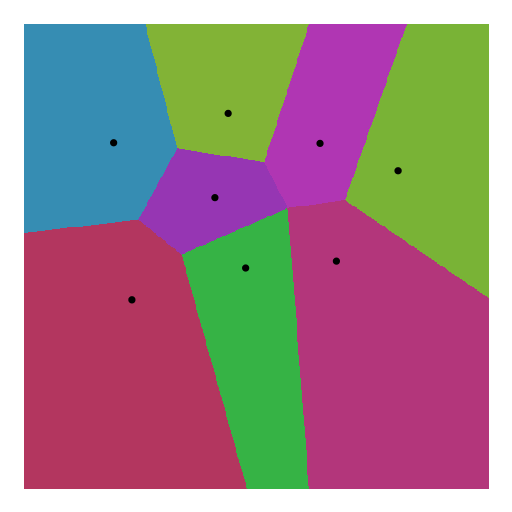
\includegraphics[scale=0.55]{pictures/kmeans_8_neuronow_zbior_0.png}
	\label{fig:kmeans_8_neuronow_zbior_0}
	\caption{Wynikowa mozaika Woronoja dla algorytmu k-średnich na zbiorze nr 1}
\end{figure}

\begin{figure}[h]
	\centering
		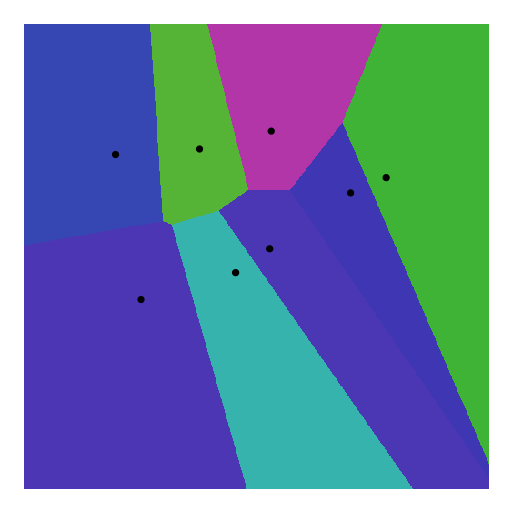
\includegraphics[scale=0.55]{pictures/kohonen_8_neuronow_zbior_0.png}
	\label{fig:kohonen_8_neuronow_zbior_0}
	\caption{Wynikowa mozaika Woronoja dla algorytmu Kohonena na zbiorze nr 1}
\end{figure}

\begin{figure}[h]
	\centering
		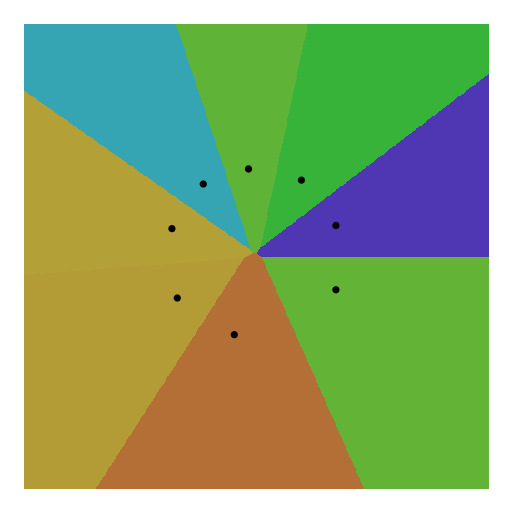
\includegraphics[scale=0.55]{pictures/kohonen_8_neuronow_zbior_0_normalized.png}
	\label{fig:kohonen_8_neuronow_zbior_0_normalized}
	\caption{Wynikowa mozaika Woronoja dla algorytmu Kohonena z normalizacją na zbiorze nr 1}
\end{figure}

\begin{figure}[h]
	\centering
		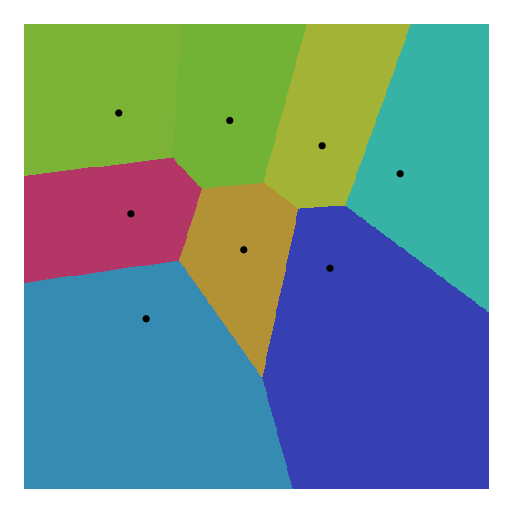
\includegraphics[scale=0.55]{pictures/neuralgas_8_neuronow_zbior_0.png}
	\label{fig:neuralgas_8_neuronow_zbior_0}
	\caption{Wynikowa mozaika Woronoja dla algorytmu gazu neuronowego na zbiorze nr 1}
\end{figure}

\begin{figure}[h]
	\centering
		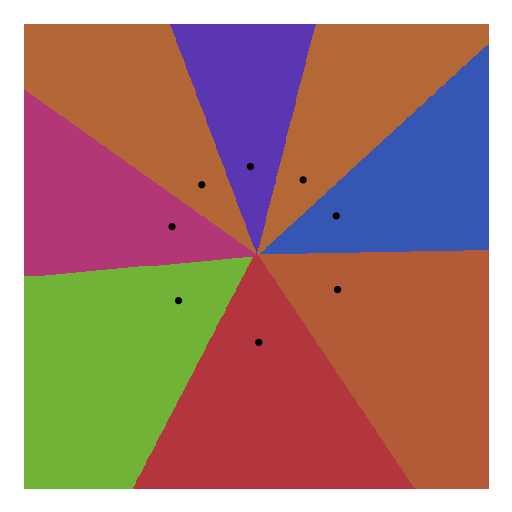
\includegraphics[scale=0.55]{pictures/neuralgas_8_neuronow_zbior_0_normalized.png}
	\label{fig:neuralgas_8_neuronow_zbior_0_normalized}
	\caption{Wynikowa mozaika Woronoja dla algorytmu gazu neuronowego z normalizacją na zbiorze nr 1}
\end{figure}

\begin{figure}[h]
	\centering
		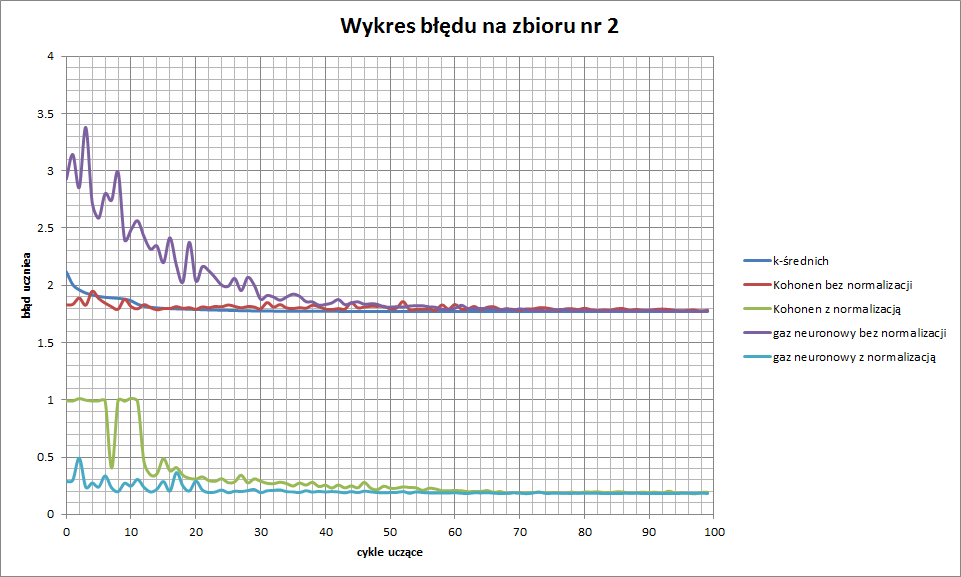
\includegraphics[scale=0.55]{pictures/183566_2.png}
	\label{fig:183566_2}
	\caption{Porównanie błędu uczenia dla zbioru danych nr 2}
\end{figure}

\begin{figure}[h]
	\centering
		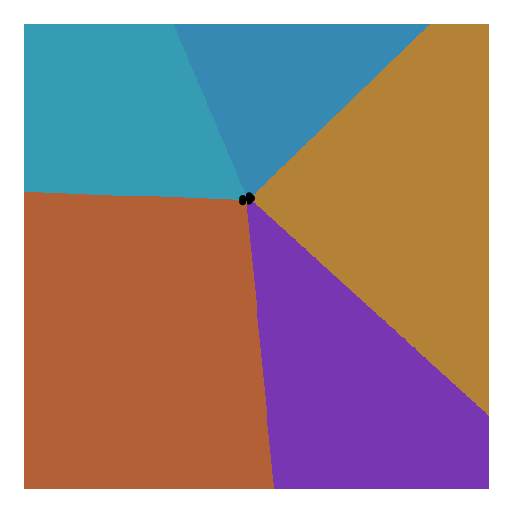
\includegraphics[scale=0.55]{pictures/kmeans_8_neuronow_zbior_1.png}
	\label{fig:kmeans_8_neuronow_zbior_1}
	\caption{Wynikowa mozaika Woronoja dla algorytmu k-średnich na zbiorze nr 2}
\end{figure}

\begin{figure}[h]
	\centering
		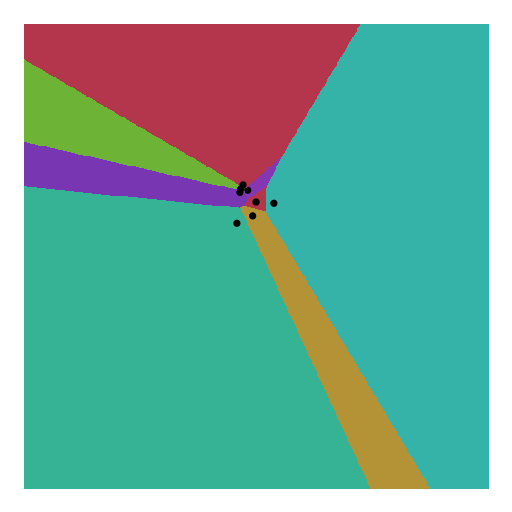
\includegraphics[scale=0.55]{pictures/kohonen_8_neuronow_zbior_1.png}
	\label{fig:kohonen_8_neuronow_zbior_1}
	\caption{Wynikowa mozaika Woronoja dla algorytmu Kohonena na zbiorze nr 2}
\end{figure}

\begin{figure}[h]
	\centering
		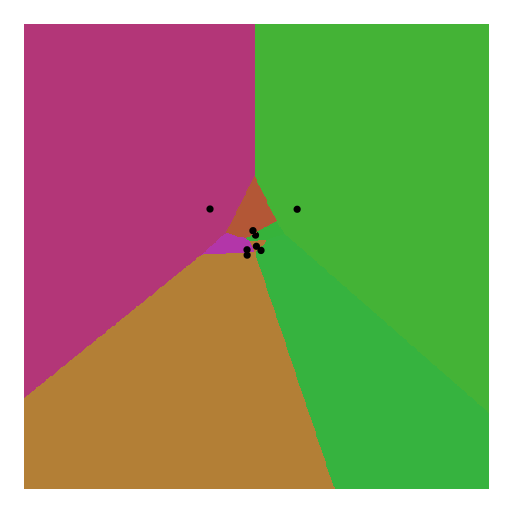
\includegraphics[scale=0.55]{pictures/kohonen_8_neuronow_zbior_1_normalized.png}
	\label{fig:kohonen_8_neuronow_zbior_1_normalized}
	\caption{Wynikowa mozaika Woronoja dla algorytmu Kohonena z normalizacją na zbiorze nr 2}
\end{figure}

\begin{figure}[h]
	\centering
		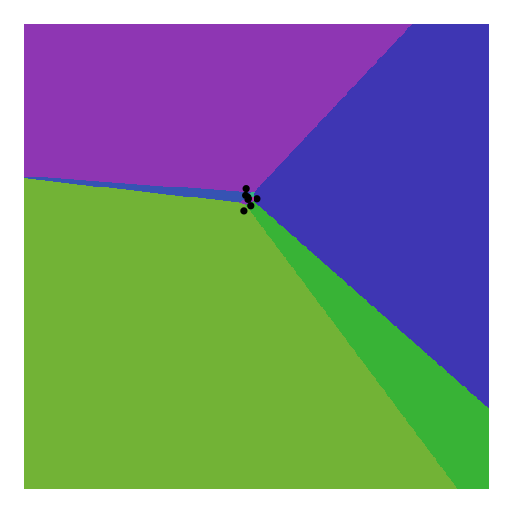
\includegraphics[scale=0.55]{pictures/neuralgas_8_neuronow_zbior_1.png}
	\label{fig:neuralgas_8_neuronow_zbior_1}
	\caption{Wynikowa mozaika Woronoja dla algorytmu gazu neuronowego na zbiorze nr 2}
\end{figure}

\begin{figure}[h]
	\centering
		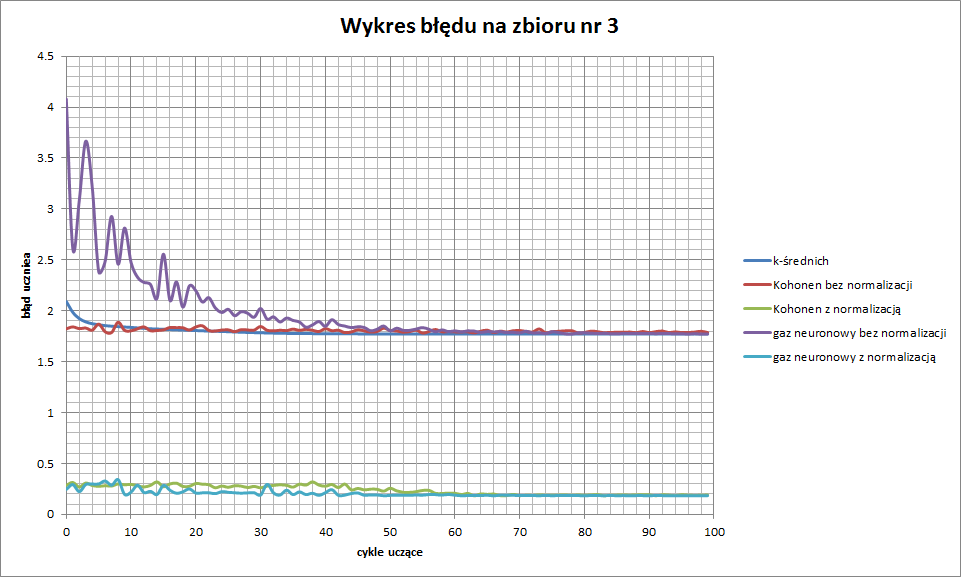
\includegraphics[scale=0.55]{pictures/183566_3.png}
	\label{fig:183566_3}
	\caption{Porównanie błędu uczenia dla zbioru danych nr 3}
\end{figure}

\begin{figure}[h]
	\centering
		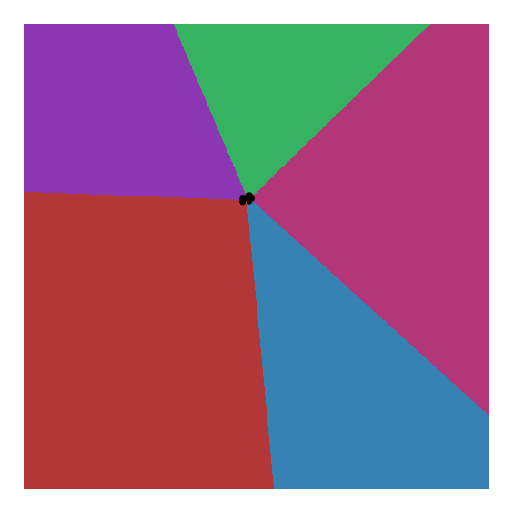
\includegraphics[scale=0.55]{pictures/kmeans_8_neuronow_zbior_2.png}
	\label{fig:kmeans_8_neuronow_zbior_2}
	\caption{Wynikowa mozaika Woronoja dla algorytmu k-średnich na zbiorze nr 3}
\end{figure}

\begin{figure}[h]
	\centering
		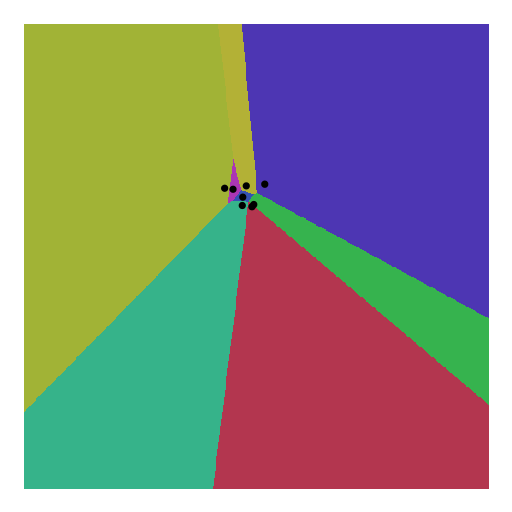
\includegraphics[scale=0.55]{pictures/kohonen_8_neuronow_zbior_2.png}
	\label{fig:kohonen_8_neuronow_zbior_2}
	\caption{Wynikowa mozaika Woronoja dla algorytmu Kohonena na zbiorze nr 3}
\end{figure}

\begin{figure}[h]
	\centering
		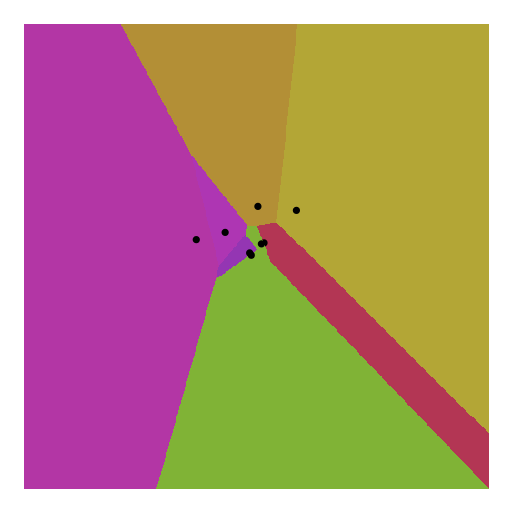
\includegraphics[scale=0.55]{pictures/kohonen_8_neuronow_zbior_2_normalized.png}
	\label{fig:kohonen_8_neuronow_zbior_2_normalized}
	\caption{Wynikowa mozaika Woronoja dla algorytmu Kohonena z normalizacją na zbiorze nr 3}
\end{figure}

\begin{figure}[h]
	\centering
		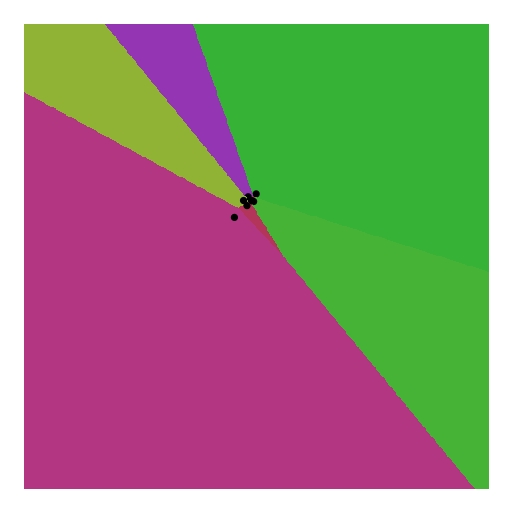
\includegraphics[scale=0.55]{pictures/neuralgas_8_neuronow_zbior_2.png}
	\label{fig:neuralgas_8_neuronow_zbior_2}
	\caption{Wynikowa mozaika Woronoja dla algorytmu gazu neuronowego na zbiorze nr 3}
\end{figure}

\clearpage
Analiza danych dla indeksu: 173524


\begin{figure}[h]
	\centering
		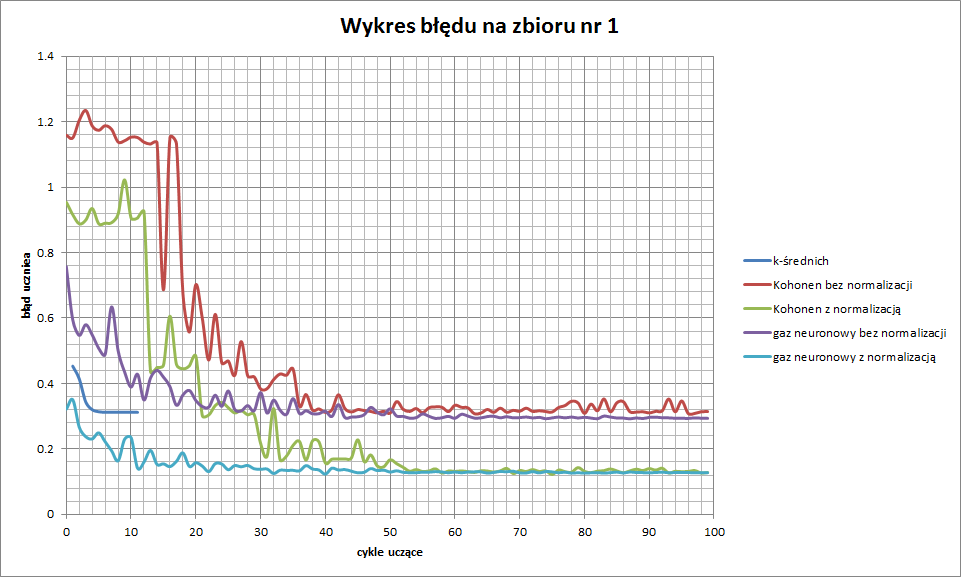
\includegraphics[scale=0.55]{pictures/173524_1.png}
	\label{fig:173524_1}
	\caption{Porównanie błędu uczenia dla zbioru danych nr 1}
\end{figure}

\begin{figure}[h]
	\centering
		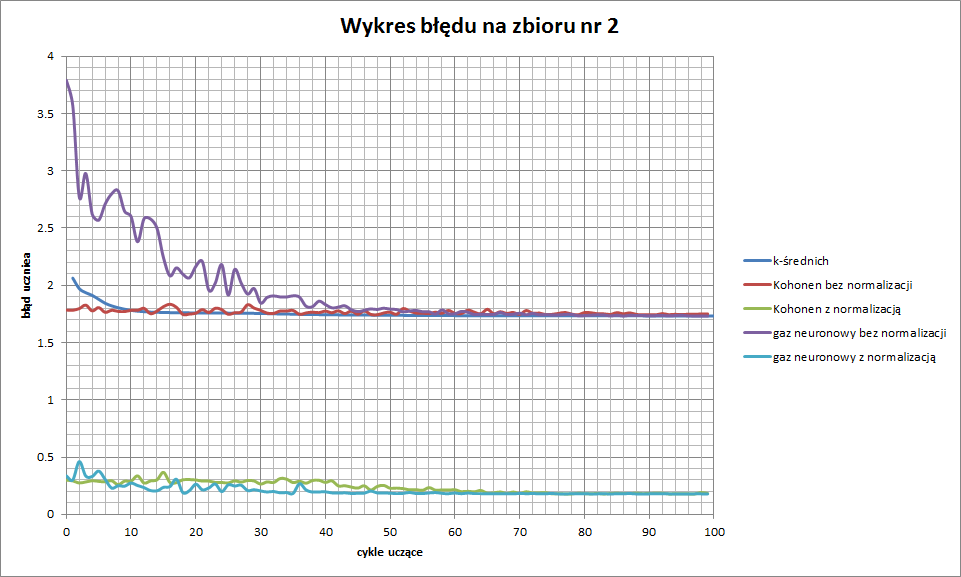
\includegraphics[scale=0.55]{pictures/173524_2.png}
	\label{fig:173524_2}
	\caption{Porównanie błędu uczenia dla zbioru danych nr 2}
\end{figure}

\begin{figure}[h]
	\centering
		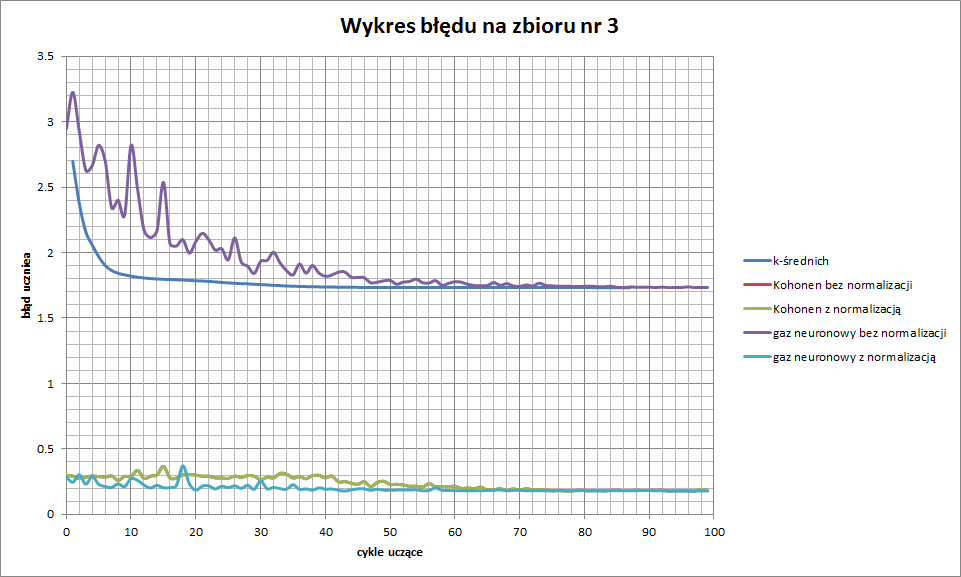
\includegraphics[scale=0.55]{pictures/173524_3.png}
		\caption{Porównanie błędu uczenia dla zbioru danych nr 3}
	\label{fig:173524_3}
\end{figure}

\clearpage

\begin{thebibliography}{0}
  \bibitem{l2short} \textsl{Stanisław Osowski} - Sieci neuronowe do przetwarzania informacji, \textsl{Wyd. 2., Warszawa 2006}
  \bibitem{l2short} ``Learning and neural networks'' [\url{http://en.wikiversity.org/wiki/Learning_and_neural_networks}]
  \bibitem{l2short} UCI Machine Learning Repository \textsl{Iris Data Set}
\end{thebibliography}
\end{document}